% IISEC 2027 submission (IEEE conference template, A4, two columns, at most 6 pages, anonymized for review).
% English version of bildiri.tex; same protocol, same numbers.
% Build: cd bildiri && latexmk -pdf paper_en.tex
% Figures and table rows: python3 scripts/bildiri_figures.py en
\documentclass[conference,a4paper]{IEEEtran}
\usepackage[T1]{fontenc}
\usepackage[utf8]{inputenc}
\usepackage{amsmath,amssymb}
\usepackage{graphicx}
\usepackage{booktabs}
\usepackage{cite}
\usepackage{url}
\newcommand{\tri}{\operatorname{tri}}
\makeatletter\newcommand{\tablerows}[1]{\@@input #1 }\makeatother

\begin{document}

\title{Loss of Plasticity in Continual Learning and Bounded Weight Reparameterizations:
A Preliminary Study of Sine, Tanh and Triangle-Wave Maps}

\author{\IEEEauthorblockN{Author information removed for double-blind review}}

\maketitle

\begin{abstract}
Neural networks trained on a long sequence of tasks gradually lose the ability to learn new ones. This is called loss of plasticity. Growth of the weight magnitude is one known cause, and keeping the weights inside a fixed interval is known to help. This preliminary study tests whether keeping the weights bounded is enough. Each weight is written as a bounded function of a free parameter. A smooth periodic map (sine), a smooth nonperiodic map (tanh) and a piecewise-linear periodic map (triangle wave) are compared with the standard network and with
weight clipping. On Online Permuted MNIST with a 200-task stream and up to ten paired seeds, the smooth maps are
slightly better than the standard network but do not preserve plasticity (retention ratio 0.93 versus 0.91).
Their weights move toward the bound, where the derivative of the map goes to zero, and the mean step
multiplier falls from 0.85 to 0.56 for sine and from 0.74 to 0.47 for tanh. The triangle wave, whose derivative has magnitude one except at its corner points, shows no loss (retention ratio 1.02). Its results did not differ from those of weight clipping, and it was not better. The findings are limited to one
dataset, a small network and a short stream.
\end{abstract}

\begin{IEEEkeywords}
continual learning, loss of plasticity, weight reparameterization, weight clipping, triangle wave
\end{IEEEkeywords}

% ----------------------------------------------------------------------------------------------------
\section{Introduction}

In continual learning a network is trained on an endless stream of tasks and is expected to learn the
thousandth task as well as the first. Standard networks trained with backpropagation do not meet this
expectation: after enough tasks they learn new tasks more slowly, and to a lower accuracy, than a freshly
initialized network \cite{ash2020warm,lyle2023understanding,dohare2024loss}. This is called \emph{loss of plasticity}. It differs from catastrophic forgetting, which is about old tasks; loss of plasticity is about learning new tasks.

Several causes have been proposed: dead or dormant units \cite{sokar2023dormant,abbas2023loss}, a falling
representation rank \cite{lyle2022understanding,dohare2024loss} and growth of the weight magnitude
\cite{dohare2024loss,elsayed2024weight,lyle2024normalization}. These causes are separate, and removing only one of them is not always enough \cite{lyle2024disentangling}. Among the methods that limit the weight magnitude, the simplest is \emph{weight
clipping} \cite{elsayed2024weight}: after every update each weight is projected back into the interval
$[-\kappa b,\kappa b]$, whose width is set by the initialization scale $b$ of the layer.

Clipping is an operation applied \emph{after} the optimizer step. The same constraint can also be built \emph{into the model}, by writing each weight as a bounded function of a free parameter:
\begin{equation}
  W = A\, f(\Theta/A), \qquad f:\mathbb{R}\to[-1,1]. \label{eq:reparam}
\end{equation}
The condition $|W|\le A$ then holds for every value of $\Theta$ and no projection step is needed. The initial
hypothesis of this work was that the choice $f=\sin$ would preserve plasticity because it keeps the weights
bounded. The experiments did not support this hypothesis. This paper reports, with preliminary results on a
short stream, why the hypothesis fails and which map works.

The contributions are as follows. (i)~Smooth bounded maps (sine, tanh) are shown, with ten paired seeds, not to
preserve plasticity on a 200-task stream. (ii)~Measurements show that this is consistent with a smaller update step, caused by the derivative of the map shrinking near the bound. (iii)~A periodic map whose derivative
does not approach zero (the triangle wave) shows no loss and gives the same result as weight clipping. The study
does not propose a method that improves on weight clipping; the contribution is an observation from experiments about
\emph{which property} of a bounded parameterization matters.

% ----------------------------------------------------------------------------------------------------
\section{Related Work}

Warm-started networks have been shown to generalize worse than networks trained from scratch \cite{ash2020warm},
and this effect grows over long task sequences \cite{dohare2024loss}. Methods that
control the weight magnitude include regularization toward the initial parameters \cite{kumar2023maintaining},
norm projection after normalization \cite{lyle2024normalization} and weight clipping \cite{elsayed2024weight}.
Lyle et al. \cite{lyle2024disentangling} report that the causes are independent of each other and that layer normalization combined with weight decay is effective at maintaining plasticity in a variety of tasks.

Periodic functions have been studied in continual learning as \emph{activations}: using sine and cosine together
in every layer kept networks trainable \cite{lewandowski2025fourier}, and plasticity has been related to the
derivative of the activation staying away from zero \cite{lillo2026activation}. A classical network with sine
activations and unbounded weights, on the other hand, has been reported to lose plasticity
\cite{chen2026intrinsic}. These studies change the function computed by a unit. Here the periodic map is
applied to the \emph{weights}: in terms of $W$ the network remains a standard rectified linear unit (ReLU) network, and only the
coordinates in which the optimizer moves change. Writing the weights as a function of other parameters changes the conditioning of the optimization problem \cite{salimans2016weight}. The triangle wave is
not new as a map with constant gradient magnitude; it was preferred to the sine in a neural shape
parameterization \cite{dai2025shaping}. In our literature search we did not find a study that applies a bounded
periodic reparameterization to network weights in the context of loss of plasticity; the search was not a systematic review.

% ----------------------------------------------------------------------------------------------------
\section{Method}

\subsection{Bounded reparameterization}

The weights of a fully connected layer with $n$ inputs are initialized uniformly in $[-b,b]$ with $b=\sqrt{6/n}$, which gives the variance $2/n$ proposed by He et al. \cite{he2015delving}. The amplitude is fixed to $A=\gamma b$ ($\gamma\ge1$), and every
weight and every bias is tied to a free parameter $\Theta$ through \eqref{eq:reparam}. Three maps are examined
(Fig.~\ref{fig:maps}):
\begin{align}
  \text{sine:}\quad & f(x)=\sin x, & f'(x)&=\cos x, \nonumber\\
  \text{tanh:}\quad & f(x)=\tanh x, & f'(x)&=1-\tanh^2 x, \nonumber\\
  \text{triangle:}\quad & f(x)=\tri(x), & |f'(x)|&=1 .
\end{align}
Here $\tri(x)=\tfrac{2}{\pi}\arcsin(\sin(\tfrac{\pi}{2}x))$ is the triangle wave with period 4; it equals the
identity on $[-1,1]$ and reflects at $\pm1$. Its derivative is $+1$ on the rising segments and $-1$ on the
falling segments and is undefined at the corner points, where the right derivative is used in the
implementation. All models start from the same effective weights: $W_0$ is drawn once and
$\Theta_0=A f^{-1}(W_0/A)$ is used.

\begin{figure}[t]
  \centering
  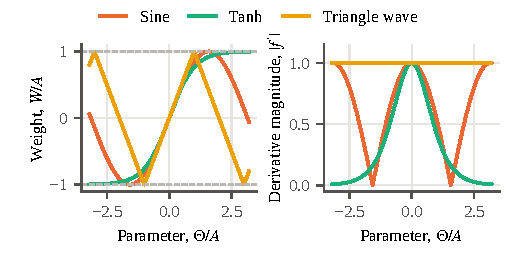
\includegraphics[width=\linewidth]{figures/fig_maps.pdf}
  \caption{The three bounded maps (left) and the magnitude of their derivatives (right). The derivative of the
  smooth maps goes to zero at the bound; that of the triangle wave is one away from the corner points.}
  \label{fig:maps}
\end{figure}

\subsection{Jacobian damping}

Let $L$ be the loss and $g=\partial L/\partial W$. A stochastic gradient step on $\Theta$ with learning rate $\eta$ changes the
effective weight, to first order, by
\begin{equation}
  \Delta W \approx f'(\Theta/A)\,\Delta\Theta = -\eta\, f'(\Theta/A)^2\, g . \label{eq:damping}
\end{equation}
The factor $f'^2\in[0,1]$ is a separate learning-rate multiplier for each parameter; it is called the
\emph{step multiplier} in this paper. For the sine map it equals $\cos^2(\Theta/A)=1-(W/A)^2$: the closer a
weight is to the bound, the smaller its step.

If a differentiable $f$ reaches its bound, it has a maximum or a minimum at that point, so the derivative is zero there. A map therefore cannot at the same time be smooth, reach its bound and have a derivative that stays away from zero. A smooth bounded map either reaches its bound (sine), in which case the step multiplier becomes zero at a finite value of $\Theta$, or only gets closer to the bound without reaching it (tanh), in which case the multiplier keeps shrinking as $|\Theta|$ grows. In both cases a weight that the data push toward the
bound slows down exactly when it gets there, and its return is made with the same small steps. Giving up smoothness removes this limit: the triangle wave is bounded and has $|f'|=1$ away from the corners.

\subsection{Reflection and projection}\label{sec:reflection}

For the triangle wave, \eqref{eq:damping} gives exactly $\Delta W=-\eta g$ inside the interval. A step that
would carry the weight to $A+\delta$ ($0<\delta<2A$) leaves it at $A-\delta$: the weight is \emph{reflected} at
the bound. Weight clipping maps the same step to $A$: the weight is \emph{projected}. After a single step from
a common starting point the two outcomes differ by at most $\delta\le\eta|g|$, and neither method rescales the
gradient. When the steps are small relative to the width of the interval, the triangle wave and clipping with
$\kappa=\gamma$ are expected to follow nearby paths in $W$ space.

% ----------------------------------------------------------------------------------------------------
\section{Experimental Setup}

\textbf{Stream.} Online Permuted MNIST \cite{goodfellow2013empirical,zenke2017continual,dohare2024loss} is used:
each task applies a new random permutation to the pixels of the MNIST images \cite{lecun1998gradient}. The
stream consists of 200 tasks; in each task 5,000 images drawn at random from the training set are presented one
at a time (batch size one) and once only. Neither task boundaries nor task identities are given to the network.
A run consists of $10^6$ updates.

\textbf{Network and optimizer.} A ReLU multilayer perceptron with three hidden layers of 100 units each is
trained with plain stochastic gradient descent.

\textbf{Models.} Five models are compared: (i)~the standard network; (ii--iv)~reparameterization of all weights and biases with the sine,
tanh and triangle-wave maps; (v)~weight clipping \cite{elsayed2024weight}.

\textbf{Hyperparameters.} All values were selected on a separate 100-task development stream (one seed), generated with a different random seed from the evaluation streams, and were not changed during evaluation. The selected values are: a
learning rate of 0.003 for all models; $\gamma=1.5$ for sine and tanh; $\gamma=1$ for the triangle wave;
$\kappa=1$ for clipping.

\textbf{Metrics.} The performance measure is the \emph{online accuracy}: the fraction of images classified
correctly before the update with that image is made. The area under the accuracy curve (\emph{AUC}) is reported as the mean online accuracy over all tasks.
The \emph{early} and \emph{final windows} are the means over the first and last 20 tasks; the \emph{retention
ratio} is the final window divided by the early window. The \emph{fresh-model gap} is the online accuracy of a
freshly initialized network on the last task minus that of the continually trained network; a positive value
means that the continually trained network is worse than a network that has seen no other task. As mechanism
measures we record the mean step multiplier $\langle f'^2\rangle$, the fraction of saturated parameters
($|f'|<0.1$), the mean weight magnitude, the norm of the actual weight step and the effective rank
\cite{roy2007effective} of the last hidden-layer representation.

\textbf{Seeds and statistics.} Ten seeds were run for the standard network and the three maps, and five for
weight clipping. A seed determines both the initialization and the permutation sequence; since the models are
compared on identical streams, all differences are paired. Means are reported with 95\% $t$-intervals over
seeds and differences with paired $t$-tests. Because the absence of a significant difference between the
triangle wave and weight clipping is not evidence of equality, two one-sided tests (TOST)
\cite{schuirmann1987comparison} with an equivalence margin of 0.005 were applied.

% ----------------------------------------------------------------------------------------------------
\section{Results}

\subsection{Performance}

\begin{figure}[t]
  \centering
  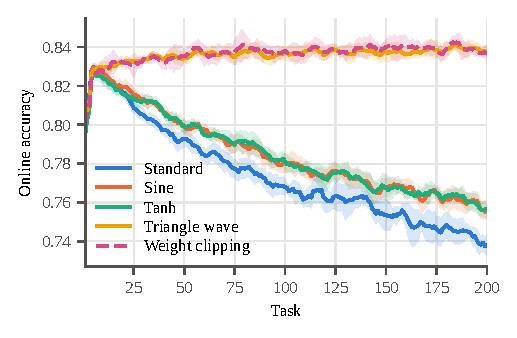
\includegraphics[width=\linewidth]{figures/fig_accuracy.pdf}
  \caption{Online accuracy on the 200-task stream (mean and 95\% interval over seeds; five-task moving
  average). The triangle-wave and weight-clipping curves overlap.}
  \label{fig:accuracy}
\end{figure}

\begin{table}[t]
  \centering
  \caption{Results on the 200-task stream (mean $\pm$ 95\% interval over ten seeds; five seeds for weight clipping).}
  \label{tab:results}
  \setlength{\tabcolsep}{2.5pt}\footnotesize
  \resizebox{\linewidth}{!}{%
  \begin{tabular}{@{}lcccc@{}} \toprule Model & AUC & Final window & Retention ratio & Fresh-model gap\\
    \midrule
    \tablerows{table_results.tex}
    \bottomrule
  \end{tabular}}
\end{table}

Fig.~\ref{fig:accuracy} and Table~\ref{tab:results} summarize the results. The online accuracy of the standard
network falls along the stream: the final window is 0.906 times the early window, and on the last task a
freshly initialized network reaches an accuracy 0.021 higher than the continually trained one.

The sine and tanh models are slightly better than the standard network: the AUC differences are $+0.0110$
(95\% interval $[+0.0100,+0.0120]$) and $+0.0109$ ($[+0.0095,+0.0123]$), positive in ten of ten seeds. Both models still lose plasticity: their retention ratios are 0.926 and 0.931, and their curves fall in
parallel with that of the standard network. No AUC difference was found between sine and tanh ($+0.0001$,
$p=0.87$).

The triangle wave shows no decline. Its retention ratio is 1.017; that is, the accuracy over the last 20 tasks
is slightly higher than over the first 20. The AUC difference is $+0.0616$ ($[+0.0595,+0.0636]$) relative to
the standard network and $+0.0506$ ($[+0.0486,+0.0525]$) relative to sine, positive in ten of ten seeds in both
comparisons. On the last task the continually trained triangle-wave network is 0.080 better than a freshly
initialized one, which suggests positive transfer from earlier tasks.

The differences between the triangle wave and weight clipping, on the five common seeds, are $+0.0004$
($[-0.0025,+0.0034]$) for AUC and $+0.0007$ ($[-0.0029,+0.0043]$) for the final window. With a margin of 0.005,
TOST indicates equivalence for AUC ($p=0.006$) and the final window ($p=0.015$) but not for the retention ratio
($p=0.052$). The two methods could not be distinguished in this experiment; there is no evidence that the
triangle wave improves on weight clipping.

\subsection{Mechanism}

\begin{figure}[t]
  \centering
  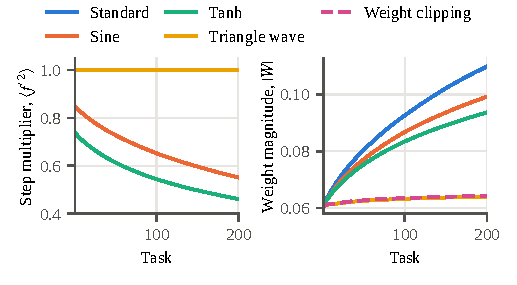
\includegraphics[width=\linewidth]{figures/fig_mechanism.pdf}
  \caption{Left: mean step multiplier $\langle f'^2\rangle$. Right: mean weight magnitude. Mean and 95\%
  interval; measurements are taken every five tasks.}
  \label{fig:mechanism}
\end{figure}

\begin{table}[t]
  \centering
  \caption{Mechanism measures. $\langle f'^2\rangle$ and the saturated fraction are means over the final window; arrows show the change from the early window to the final window; the step norm is the final-window value divided by the early-window value.}
  \label{tab:mechanism}
  \setlength{\tabcolsep}{2.5pt}\footnotesize
  \resizebox{\linewidth}{!}{%
  \begin{tabular}{@{}lccccc@{}}
    \toprule
    Model & $\langle f'^2\rangle$ & Saturated (\%) & Mean $|W|$ & Step norm & Effective rank\\
    \midrule
    \tablerows{table_mechanism.tex}
    \bottomrule
  \end{tabular}}
\end{table}

Fig.~\ref{fig:mechanism} and Table~\ref{tab:mechanism} show that the loss in the smooth maps is consistent
with \eqref{eq:damping}. In the sine and tanh models the mean weight magnitude grows along the stream (from
0.064 to 0.098 and 0.093); as the weights approach the bound the mean step multiplier falls steadily: for sine from 0.85 at the first measurement to 0.56 in the final window, and for tanh from 0.74 to 0.47. In line with this, the norm of the actual weight step
drops to 0.85 and 0.84 times its early-window value; for the standard network, the triangle wave and weight
clipping this ratio is slightly above one. At this stream length the fraction of fully saturated parameters
($|f'|<0.1$) is still low (4.3\% for sine); the loss appears together with a slowdown spread over all
parameters rather than with a small number of frozen ones.

For the triangle wave the step multiplier is one by definition and the mean weight magnitude stays almost
constant along the stream (from 0.061 to 0.064); the same values are measured for weight clipping. The
effective rank of the last hidden-layer representation falls from 37 to 22 in the standard network and from 34
to 21 for sine, whereas it does not fall for the triangle wave and weight clipping (from 33 to 37 and 38). The
fraction of dead units is similar across the models (between 0.12 and 0.18 in the final window) and does
not explain the observed difference.

% ----------------------------------------------------------------------------------------------------
\section{Discussion and Limitations}

The results suggest that, in this experimental setting, bounding each weight is not enough on its own: in the sine and tanh models the weights are bounded by construction, but the loss of plasticity remains. What the two methods that work (triangle wave, weight clipping) have in common is that
they keep the bound without shrinking the update. The small advantage of the smooth maps over the standard
network may be explained by the bound slowing the growth of the weights; the same bound, however, also shrinks
the steps.

That the triangle wave and weight clipping could not be distinguished agrees with the expectation of
Section~\ref{sec:reflection}: for small steps the difference between reflection and projection does not exceed
the size of a single step. The possible advantage of the triangle wave lies not in performance but in the
constraint being part of the model; whether this brings any practical benefit was not tested in this study.

The study has the following limitations. (i)~A single dataset and a small fully connected network are used.
(ii)~The stream is short (200 tasks, 5,000 samples per task); longer streams are needed to see a loss that builds up slowly. (iii)~Only stochastic gradient descent is tried; with adaptive optimizers the step
may be large relative to the interval, so the results may differ. (iv)~The width of the bound differs between
the models (it was selected separately for each model on the development stream); the effects of the shape of
the map and of the width of the bound are therefore not fully separated in this experiment. (v)~Weight clipping
was run with five seeds. (vi)~That the damping is the \emph{cause} of the loss is not tested directly here; the
measurements are only consistent with this explanation. An intervention experiment that changes only the
backward derivative while leaving the forward map unchanged, and experiments on longer streams, are in progress.

% ----------------------------------------------------------------------------------------------------
\section{Conclusion}

On a 200-task Online Permuted MNIST stream, bounding the weights with a smooth map (sine, tanh) did not prevent
loss of plasticity; in these models the mean step multiplier fell by about one third along the stream. The
triangle-wave map, whose derivative does not approach zero, showed no loss and gave the same result as weight
clipping. These preliminary findings suggest that, in a bounded weight parameterization, keeping the size of the update matters as well as keeping the weights bounded. Whether the findings hold on longer streams, on other
datasets and with other optimizers remains to be tested.

\section*{Acknowledgment}

An AI assistant (Claude, Anthropic) was used in this work to help write and run the experiment and analysis code, to
produce the figures and tables from the experiment logs, and to draft and edit the text of all sections. The authors
directed the work, reviewed all content and take full responsibility for it.

\bibliographystyle{IEEEtran}
\bibliography{kaynaklar}

\end{document}
